\documentclass[11pt,a4paper]{article}

% Packages
\usepackage[utf8]{inputenc}
\usepackage[T1]{fontenc}
\usepackage[brazilian]{babel}
\usepackage{lmodern}
\usepackage[a4paper,margin=2.5cm]{geometry}
\usepackage{amsmath}
\usepackage{graphicx}
\usepackage{rotating}
\usepackage{float}
\usepackage{array}
\usepackage{longtable}
\usepackage{enumitem}
\usepackage{needspace}
\usepackage[hidelinks]{hyperref}

\graphicspath{{figuras/}}
\setlength{\parindent}{0pt}
\setlength{\parskip}{4pt}

% \casodeuso{título}
\newcommand{\casodeuso}[1]{\subsection{Caso de Uso: #1}}
\newcommand{\campo}[1]{\textbf{#1:}~}

% Cabeçalhos dos blocos de fluxo
\newcommand{\fluxotitulo}[1]{\par\needspace{8\baselineskip}\medskip\hspace*{1.5em}\textbf{#1}\par\nopagebreak}
\newcommand{\subfluxo}[1]{\par\needspace{4\baselineskip}\smallskip\hspace*{1.5em}\textbf{#1}\par\nopagebreak}

% Lista numerada do fluxo principal
\newenvironment{principal}
  {\begin{enumerate}[leftmargin=4.5em,itemsep=0pt,topsep=2pt]}
  {\end{enumerate}}

% Lista de passos rotulados (A1.1, E1.2, ...)
\newenvironment{passos}
  {\begin{description}[leftmargin=4.5em,labelindent=3em,itemsep=0pt,topsep=2pt,
     font=\normalfont\bfseries,style=sameline]}
  {\end{description}}
\newcommand{\passo}[1]{\item[#1 -]}

% Lista de regras de negócio / pré-condições
\newenvironment{itens}
  {\begin{itemize}[leftmargin=3em,itemsep=0pt,topsep=2pt]}
  {\end{itemize}}

\title{Trabalho Prático - Design de Software}
\author{
  BEATRIZ PONTES CAMARGO GRR20242966\\
  EDUARDO KALUF GRR20241770\\
  IGOR GALVAN GRANDO GRR20241962\\
  KAUÊ DE AMORIM SILVA GRR20244719\\
  SERGIO SIVONEI DE SANT'ANA FILHO GRR20242337}
\date{\today}

% Document
\begin{document}
  \maketitle

  \section{Engenharia de Requisitos - Trabalho Base}\label{sec:engenharia-de-requisitos---trabalho-base}

  % ---------------------------------------------------------------------------
  \subsection{Descrição do Sistema}\label{subsec:descricao-do-sistema}

  \textbf{Descrição do Sistema para a Plataforma de Ensino de Programação.}

  O sistema tem o objetivo de oferecer cursos de programação on-line, nos quais
  o aluno assiste a aulas, executa código em um compilador integrado à própria
  plataforma, sem necessidade de ferramentas externas, e resolve exercícios.
  Como objetivos secundários, acompanhar o progresso de cada aluno nos cursos e
  emitir certificados de conclusão.

  O sistema deverá permitir que um visitante se cadastre na plataforma,
  informando e-mail e senha. O sistema deverá recusar e-mails inválidos,
  temporários, de spam ou já cadastrados, e senhas que não tenham mais de 8
  caracteres ou que não contenham ao menos uma letra, um número e um símbolo. O sistema deverá permitir que o
  usuário cadastrado realize login com seu e-mail e senha, informando quando o
  e-mail não estiver cadastrado ou a senha estiver incorreta. O armazenamento e
  a validação das credenciais ficam a cargo do serviço de autenticação.

  O sistema deverá permitir que qualquer usuário cadastrado crie um curso,
  inserindo título, descrição, linguagens utilizadas e nível de dificuldade, e
  passando a ser o professor daquele curso. O curso deverá ser organizado em
  módulos, e cada módulo em aulas (com vídeo, transcrição e resumo), exercícios
  (com enunciado, código de apoio e dificuldade) e materiais de apoio para
  download. O sistema deverá validar automaticamente todo conteúdo antes de
  publicá-lo, recusando conteúdo inadequado ou não relacionado ao curso. Um
  curso que permanecer sem conteúdo deverá ser removido após 7 dias, com aviso
  prévio ao professor.

  O sistema deverá permitir que o professor gerencie o conteúdo dos seus
  cursos, adicionando, editando e removendo aulas, exercícios e materiais de apoio, com
  confirmação antes de cada remoção. Somente o criador do curso poderá alterar
  seu conteúdo, e as alterações não poderão corromper o progresso dos alunos.

  O sistema deverá permitir que o aluno realize as aulas de forma interativa:
  assistir aos vídeos ajustando a velocidade de reprodução, fazer anotações
  vinculadas à aula, favoritar aulas, executar códigos no compilador integrado
  e resolver os exercícios propostos. O sistema deverá exibir uma mensagem de
  erro quando o código não puder ser executado, informar quando uma aula estiver
  indisponível e permitir que o aluno marque como concluída uma aula que já
  tenha acessado. O progresso do aluno deverá ser salvo automaticamente.

  O sistema deverá permitir que o aluno com 100\% de progresso em um curso, isto
  é, com todas as aulas concluídas e todos os exercícios resolvidos com sucesso,
  emita e baixe um certificado digital em PDF contendo seu nome, o nome do
  curso, a carga horária e um código único de validação. O certificado deverá
  poder ser compartilhado por meio de um link público de validação. Caso o curso
  não esteja completo, o sistema deverá bloquear a emissão e listar as
  pendências do aluno. Ao concluir a última aula de um curso, o sistema deverá
  oferecer ao aluno a emissão do certificado.

  % ---------------------------------------------------------------------------
  \casodeuso{Realizar cadastro}

  \campo{Descrição} O visitante cria uma conta na plataforma.\\
  \campo{Atores} Visitante (principal); Serviço de Autenticação (secundário).\\
  \campo{Pré-Condições} O usuário não pode estar logado.

  \needspace{8\baselineskip}\campo{Fluxos}

  \fluxotitulo{Principal:}
  \begin{principal}
    \item O visitante insere seu e-mail.
    \item O visitante insere sua senha.
    \item O serviço de autenticação salva as credenciais.
    \item O visitante é encaminhado para o login e o caso de uso é encerrado.
  \end{principal}

  \fluxotitulo{Fluxos de Exceção:}
  \begin{passos}
    \passo{E1} No passo 1, o e-mail é inválido, temporário ou de spam. O
    sistema informa o visitante e o fluxo retorna ao passo 1.
    \passo{E2} No passo 1, o e-mail já está cadastrado. O sistema informa o
    visitante, pergunta se ele deseja realizar login e o fluxo retorna ao
    passo 1.
    \passo{E3} No passo 2, a senha não atende à RN01. O sistema informa o
    visitante e o fluxo retorna ao passo 2.
  \end{passos}

  \needspace{4\baselineskip}\campo{Regras de Negócio}
  \begin{itens}
    \item \textbf{RN01} -- A senha deve ter mais de 8 caracteres, contendo pelo
    menos uma letra, um número e um símbolo.
  \end{itens}

  % ---------------------------------------------------------------------------
  \casodeuso{Realizar login}

  \campo{Descrição} O usuário cadastrado entra na plataforma com seu e-mail e
  senha.\\
  \campo{Atores} Visitante (principal); Serviço de Autenticação (secundário).\\
  \campo{Pré-Condições} O usuário deve estar cadastrado e não pode estar logado.

  \needspace{8\baselineskip}\campo{Fluxos}

  \fluxotitulo{Principal:}
  \begin{principal}
    \item O visitante insere seu e-mail.
    \item O visitante insere sua senha.
    \item O serviço de autenticação valida as credenciais.
    \item O visitante é encaminhado para o menu principal e o caso de uso é
    encerrado.
  \end{principal}

  \fluxotitulo{Fluxos de Exceção:}
  \begin{passos}
    \passo{E1} No passo 3, o e-mail não está cadastrado. O sistema informa o
    visitante e o fluxo retorna ao passo 1.
    \passo{E2} No passo 3, a senha está incorreta. O sistema informa o
    visitante e o fluxo retorna ao passo 2.
  \end{passos}

  % ---------------------------------------------------------------------------
  \casodeuso{Criação de Curso}

  \campo{Descrição} O usuário cria um curso na plataforma e passa a ser o
  professor dele.\\
  \campo{Atores} Aluno (principal).\\
  \campo{Pré-Condições} O usuário deve estar logado no sistema.

  \needspace{8\baselineskip}\campo{Fluxos}

  \fluxotitulo{Principal:}
  \begin{principal}
    \item O usuário insere os dados do curso (título, descrição, linguagens
    utilizadas e nível de dificuldade).
    \item O sistema valida os dados, cria o curso e o usuário passa a ser o
    professor dele.
    \item O professor adiciona o conteúdo do curso (aulas, exercícios e
    materiais de apoio, organizados em módulos), conforme o caso de uso
    Gerenciar Conteúdo do Curso.
    \item O caso de uso é encerrado.
  \end{principal}

  \fluxotitulo{Fluxos Alternativos:}
  \begin{passos}
    \passo{A1} No passo 3, o professor não adiciona nenhum conteúdo. O sistema
    avisa que o curso será removido em 7 dias caso permaneça vazio (RN01) e o
    caso de uso é encerrado.
  \end{passos}

  \fluxotitulo{Fluxos de Exceção:}
  \begin{passos}
    \passo{E1} No passo 3, o conteúdo é classificado como inadequado ou não
    relacionado ao curso. O tratamento segue o fluxo de exceção E1 de Gerenciar
    Conteúdo do Curso.
  \end{passos}

  \needspace{4\baselineskip}\campo{Regras de Negócio}
  \begin{itens}
    \item \textbf{RN01} -- Todo curso deve ter algum conteúdo. Um curso que
    permanecer vazio é removido após 7 dias.
  \end{itens}

  % ---------------------------------------------------------------------------
  \casodeuso{Gerenciar Conteúdo do Curso}

  \campo{Descrição} O professor adiciona, edita ou remove conteúdos de um curso
  que criou.\\
  \campo{Atores} Professor (principal).\\
  \campo{Pré-Condições}
  \begin{itens}
    \item O usuário deve estar logado no sistema.
    \item O usuário deve ser o criador do curso.
  \end{itens}
  \needspace{8\baselineskip}\campo{Fluxos}

  \fluxotitulo{Principal:}
  \begin{principal}
    \item O professor acessa o painel do curso.
    \item O professor seleciona um conteúdo existente (aula, exercício ou
    material de apoio).
    \item O professor edita o conteúdo.
    \item O sistema valida as alterações (RN02).
    \item O sistema salva as alterações e mantém o conteúdo disponível aos
    alunos.
    \item O caso de uso é encerrado.
  \end{principal}

  \fluxotitulo{Fluxos Alternativos:}

  \subfluxo{A1 -- Remover conteúdo}
  \begin{passos}
    \passo{A1.1} No passo 2, o professor seleciona a opção de remover o
    conteúdo.
    \passo{A1.2} O sistema solicita confirmação.
    \passo{A1.3} O professor confirma.
    \passo{A1.4} O sistema remove o conteúdo, sem corromper o progresso dos
    alunos (RN03).
    \passo{A1.5} O caso de uso é encerrado.
  \end{passos}

  \subfluxo{A2 -- Adicionar novo conteúdo}
  \begin{passos}
    \passo{A2.1} No passo 2, o professor seleciona a opção de adicionar
    conteúdo e escolhe o módulo em que ele será inserido, podendo criar um novo
    módulo.
    \passo{A2.2} O professor insere os dados do conteúdo.
    \passo{A2.3} O fluxo segue para o passo 4.
  \end{passos}

  \fluxotitulo{Fluxos de Exceção:}

  \subfluxo{E1 -- Conteúdo inválido}
  \begin{passos}
    \passo{E1.1} No passo 4, o sistema identifica conteúdo inadequado ou não
    relacionado ao curso.
    \passo{E1.2} O sistema bloqueia a ação e informa o professor.
    \passo{E1.3} O fluxo retorna ao passo 3 para correção.
  \end{passos}

  \needspace{4\baselineskip}\campo{Regras de Negócio}
  \begin{itens}
    \item \textbf{RN01} -- Apenas o criador do curso pode adicionar, editar ou
    remover seu conteúdo.
    \item \textbf{RN02} -- Todo conteúdo deve passar por validação automática
    antes de ser publicado.
    \item \textbf{RN03} -- Alterações não podem corromper o progresso dos alunos.
  \end{itens}

  % ---------------------------------------------------------------------------
  \casodeuso{Realizar Aula Interativa}

  \campo{Descrição} O aluno acessa uma aula, consome o conteúdo e realiza
  atividades práticas, incluindo execução de código e resolução de exercícios.\\
  \campo{Atores} Aluno (principal); Compilador Integrado (secundário).\\
  \campo{Pré-Condições} O usuário deve estar logado no sistema.

  \needspace{8\baselineskip}\campo{Fluxos}

  \fluxotitulo{Principal:}
  \begin{principal}
    \item O sistema apresenta os cursos disponíveis ao aluno.
    \item O aluno seleciona um curso.
    \item O sistema exibe as aulas do curso selecionado, organizadas por módulo.
    \item O aluno seleciona uma aula.
    \item O sistema exibe o conteúdo da aula (vídeo, transcrição e resumo).
    \item O aluno executa códigos no compilador integrado.
    \item O aluno resolve os exercícios propostos.
    \item O aluno marca a aula como concluída.
    \item O sistema atualiza o progresso do aluno no curso.
    \item O caso de uso é encerrado.
  \end{principal}

  \fluxotitulo{Fluxos Alternativos:}

  \subfluxo{A1 -- Favoritar aula}
  \begin{passos}
    \passo{A1.1} O aluno seleciona a opção de favoritar a aula.
    \passo{A1.2} O sistema adiciona a aula à lista de favoritos do aluno.
    \passo{A1.3} O fluxo retorna ao passo 5.
  \end{passos}

  \subfluxo{A2 -- Fazer anotação}
  \begin{passos}
    \passo{A2.1} O aluno seleciona a opção de adicionar anotação.
    \passo{A2.2} O sistema disponibiliza um campo de texto.
    \passo{A2.3} O aluno insere a anotação.
    \passo{A2.4} O sistema salva a anotação vinculada à aula (RN03).
    \passo{A2.5} O fluxo retorna ao passo 5.
  \end{passos}

  \subfluxo{A3 -- Ajustar velocidade do vídeo}
  \begin{passos}
    \passo{A3.1} O aluno altera a velocidade de reprodução do vídeo.
    \passo{A3.2} O sistema ajusta a reprodução conforme selecionado.
    \passo{A3.3} O fluxo retorna ao passo 5.
  \end{passos}

  \subfluxo{A4 -- Curso concluído (ponto de extensão)}
  \begin{passos}
    \passo{A4.1} No passo 9, o progresso do aluno no curso chega a 100\%.
    \passo{A4.2} O sistema oferece a emissão do certificado.
    \passo{A4.3} Se o aluno aceitar, é executado o caso de uso Emitir
    Certificado de Conclusão, a partir do seu passo 3.
  \end{passos}

  \fluxotitulo{Fluxos de Exceção:}

  \subfluxo{E1 -- Erro na execução de código}
  \begin{passos}
    \passo{E1.1} No passo 6, o sistema não consegue executar o código inserido.
    \passo{E1.2} O sistema exibe uma mensagem de erro ao aluno.
    \passo{E1.3} O aluno pode corrigir o código e tentar novamente.
    \passo{E1.4} O fluxo retorna ao passo 6.
  \end{passos}

  \subfluxo{E2 -- Aula indisponível}
  \begin{passos}
    \passo{E2.1} No passo 4, o sistema identifica que a aula selecionada não
    está disponível.
    \passo{E2.2} O sistema exibe uma mensagem informando a indisponibilidade.
    \passo{E2.3} O caso de uso é encerrado.
  \end{passos}

  \needspace{4\baselineskip}\campo{Pós-Condições}
  \begin{itens}
    \item O progresso do aluno é atualizado no sistema.
    \item A aula pode ser marcada como concluída.
  \end{itens}

  \needspace{4\baselineskip}\campo{Regras de Negócio}
  \begin{itens}
    \item \textbf{RN01} -- O progresso deve ser salvo automaticamente.
    \item \textbf{RN02} -- O aluno só pode marcar a aula como concluída após
    acessá-la.
    \item \textbf{RN03} -- As anotações devem ser vinculadas à aula específica.
    \item \textbf{RN04} -- A execução de código deve ocorrer diretamente na
    plataforma, sem necessidade de ferramentas externas.
  \end{itens}

  % ---------------------------------------------------------------------------
  \casodeuso{Emitir Certificado de Conclusão}

  \campo{Descrição} O aluno solicita e baixa o certificado de um curso após
  concluir todas as suas aulas e exercícios.\\
  \campo{Atores} Aluno (principal).\\
  \campo{Pré-Condições} O usuário deve estar logado no sistema.

  \needspace{8\baselineskip}\campo{Fluxos}

  \fluxotitulo{Principal:}
  \begin{principal}
    \item O aluno acessa o painel do curso.
    \item O aluno seleciona a opção ``Emitir Certificado''.
    \item O sistema valida o progresso do aluno no curso (aulas concluídas e
    exercícios resolvidos com sucesso).
    \item O sistema gera o certificado digital (PDF) contendo o nome do aluno, o
    nome do curso, a carga horária e um código único de validação (RN02).
    \item O sistema exibe o certificado e disponibiliza a opção de download.
    \item O aluno realiza o download do arquivo.
    \item O caso de uso é encerrado.
  \end{principal}

  \fluxotitulo{Fluxos Alternativos:}

  \subfluxo{A1 -- Compartilhar validação pública}
  \begin{passos}
    \passo{A1.1} No passo 5, o aluno seleciona a opção de compartilhar o
    certificado (ex: no LinkedIn).
    \passo{A1.2} O sistema gera um link público de validação do certificado.
    \passo{A1.3} O aluno copia o link ou é redirecionado automaticamente para a
    rede social com os dados preenchidos.
    \passo{A1.4} O caso de uso é encerrado.
  \end{passos}

  \fluxotitulo{Fluxos de Exceção:}

  \subfluxo{E1 -- Curso incompleto}
  \begin{passos}
    \passo{E1.1} No passo 3, o sistema identifica que o progresso do aluno é
    inferior a 100\%.
    \passo{E1.2} O sistema informa que o certificado está bloqueado e lista as
    aulas e os exercícios pendentes.
    \passo{E1.3} O fluxo retorna ao passo 1.
  \end{passos}

  \needspace{4\baselineskip}\campo{Regras de Negócio}
  \begin{itens}
    \item \textbf{RN01} -- O certificado só pode ser gerado se o aluno tiver
    concluído todas as aulas e resolvido com sucesso todos os exercícios do
    curso (100\% de progresso).
    \item \textbf{RN02} -- O certificado deve possuir um código de validação
    único e rastreável pelo sistema, para evitar falsificações.
  \end{itens}

  % ===========================================================================
  \section{Descrição dos Atores}

  \textbf{Visitante}: Usuário não autenticado, que interage com o sistema por
  meio dos casos de uso Realizar cadastro e Realizar login.

  \textbf{Aluno}: Usuário autenticado que acessa os cursos, assiste às aulas,
  resolve exercícios e emite certificados de conclusão. As funcionalidades de
  anotações, favoritos e execução de código estão contidas no caso de uso
  Realizar Aula Interativa. Qualquer aluno pode criar um curso, passando a ser o
  professor dele.

  \textbf{Professor}: Aluno que criou ao menos um curso. De modo análogo ao dono
  de um repositório no Github, é responsável por gerenciar o conteúdo dos seus
  cursos (aulas, exercícios e materiais de apoio) e continua podendo ser aluno de
  outros cursos.

  \textbf{Serviço de Autenticação}: Responsável por armazenar e validar as
  credenciais (e-mail e senha) dos usuários nos casos de uso Realizar cadastro e
  Realizar login.

  \textbf{Compilador Integrado}: Serviço responsável por executar os códigos
  submetidos pelos alunos durante as aulas e a resolução de exercícios.

  % ===========================================================================
  \section{Diagrama de Caso de Uso}

  % Fonte editável: diagramas/diagrama-casos-de-uso.drawio
  \begin{figure}[H]
    \centering
    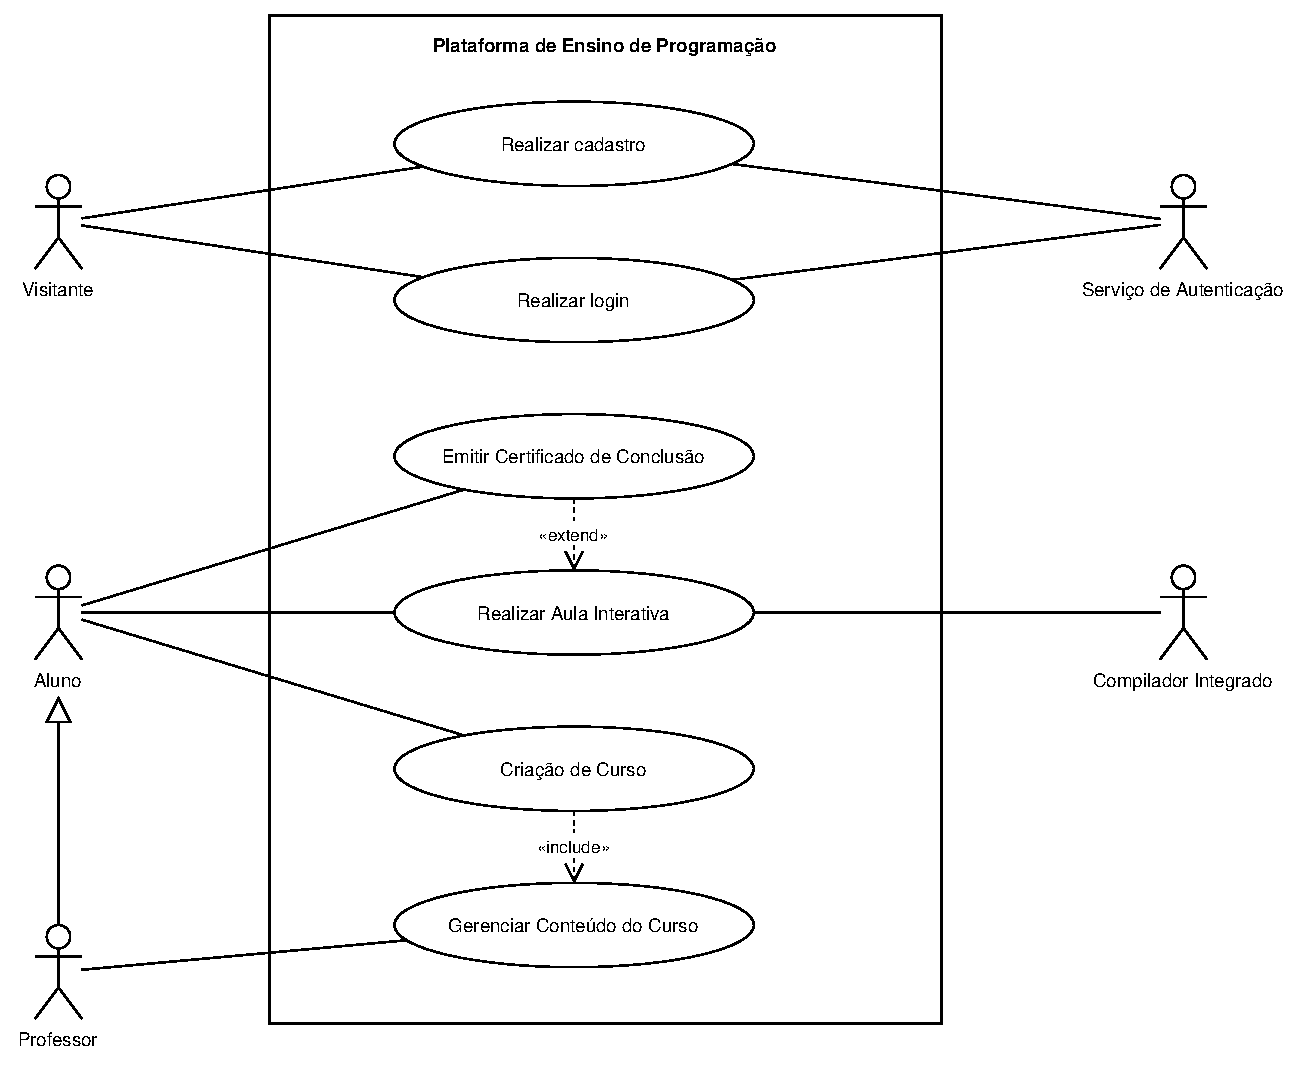
\includegraphics[width=\textwidth,height=0.8\textheight,keepaspectratio]{diagrama-casos-de-uso.pdf}
    \caption{Diagrama de casos de uso da Plataforma de Ensino de Programação.}
    \label{fig:casos-de-uso}
  \end{figure}

  % ===========================================================================
  \section{Diagrama de Classes Conceituais}

  % Fonte editável: diagramas/diagrama-classes.drawio
  \begin{figure}[H]
    \centering
    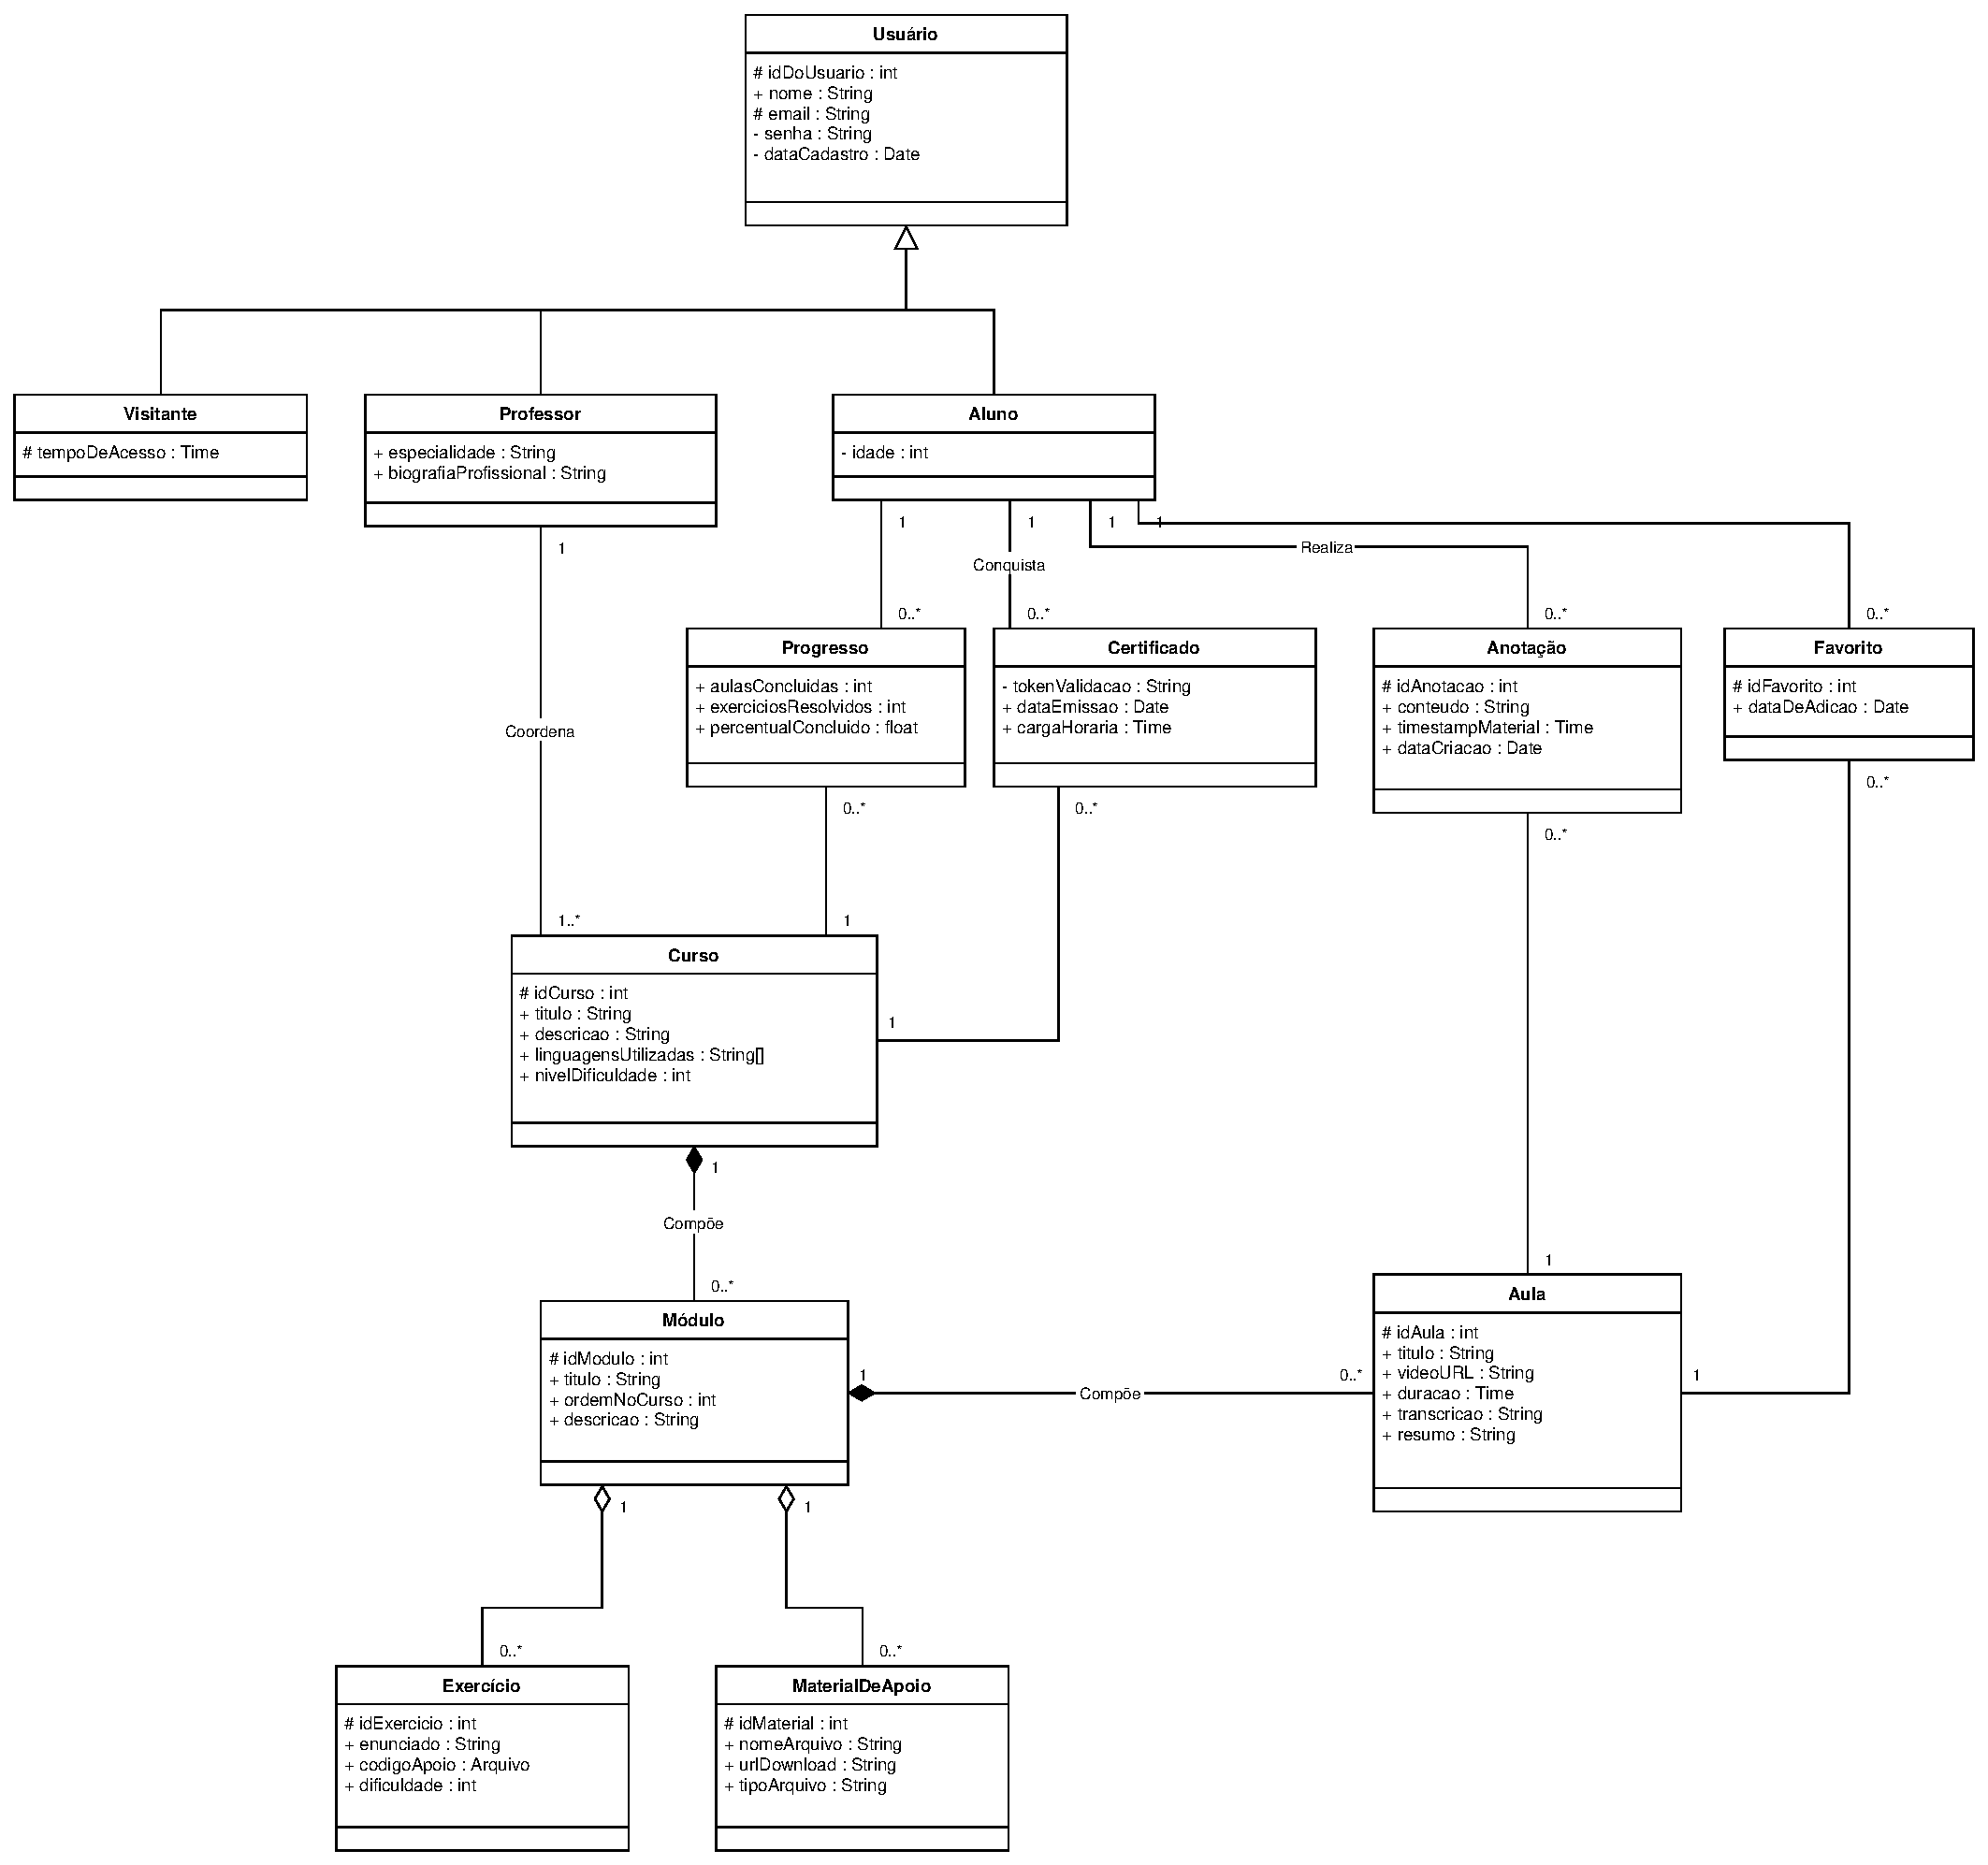
\includegraphics[width=\textwidth,height=0.8\textheight,keepaspectratio]{diagrama-classes.pdf}
    \caption{Diagrama de classes conceituais.}
    \label{fig:classes}
  \end{figure}
\end{document}
